\begin{frame}
\frametitle{About This Work...}

\emph{Spatio-temporal Joins on Symbolic Indoor Tracking Data}.~\cite{DBLP:conf/icde/LuYCJ11} \\
H.~Lu, B.~Yang, and C.~S. Jensen.\\~\\

\begin{itemize}
  \item Published at \emph{ICDE' 2011}.
  \item Studies the probabilistic, spatio-temporal joins on hisorical indoor tracking data.
  \item Two-phase hash-based algorithms are proposed for the point and interval joins.
  \item A filter-and-refine framework, along with spatial indexes and pruning rules.
\end{itemize}

\end{frame}
%------------------------------------------------

\begin{frame}
\frametitle{Motivation}

\begin{itemize}
  \item Huge amount of tracking data serves as a foundation for a wide variety of indoor applications and services.\cite{jensen2010indoor}
    \begin{fitemize}
      \item shopping mall, airports, office buildings, akin to those enabled by outdoor GPS
      \item hot area detection, space planning, security control, movement pattern discovery
    \end{fitemize}

  \item Spatio-temporal joins fall short in indoor setting.
    \begin{fitemize}
      \item indoor space consists of semantic entities enable or constrain movement
      \item semantics of indoor space call for novel spatio-temporal join predicates
      \item indoor positioning technologies differ fundamentally from outdoor setting, low accuracy and sampling frequency
    \end{fitemize}

  \item Joins on indoor tracking data call for new definition and new implementation techniques that take into account:
  \begin{fitemize}
    \item specifics of indoor space
    \item limitations of indoor positioning
  \end{fitemize}
\end{itemize}

\end{frame}
%------------------------------------------------

%------------------------------------------------

\begin{frame}
\frametitle{Preliminaries: Symbolic Indoor Tracking}

\begin{figure}[tb]
  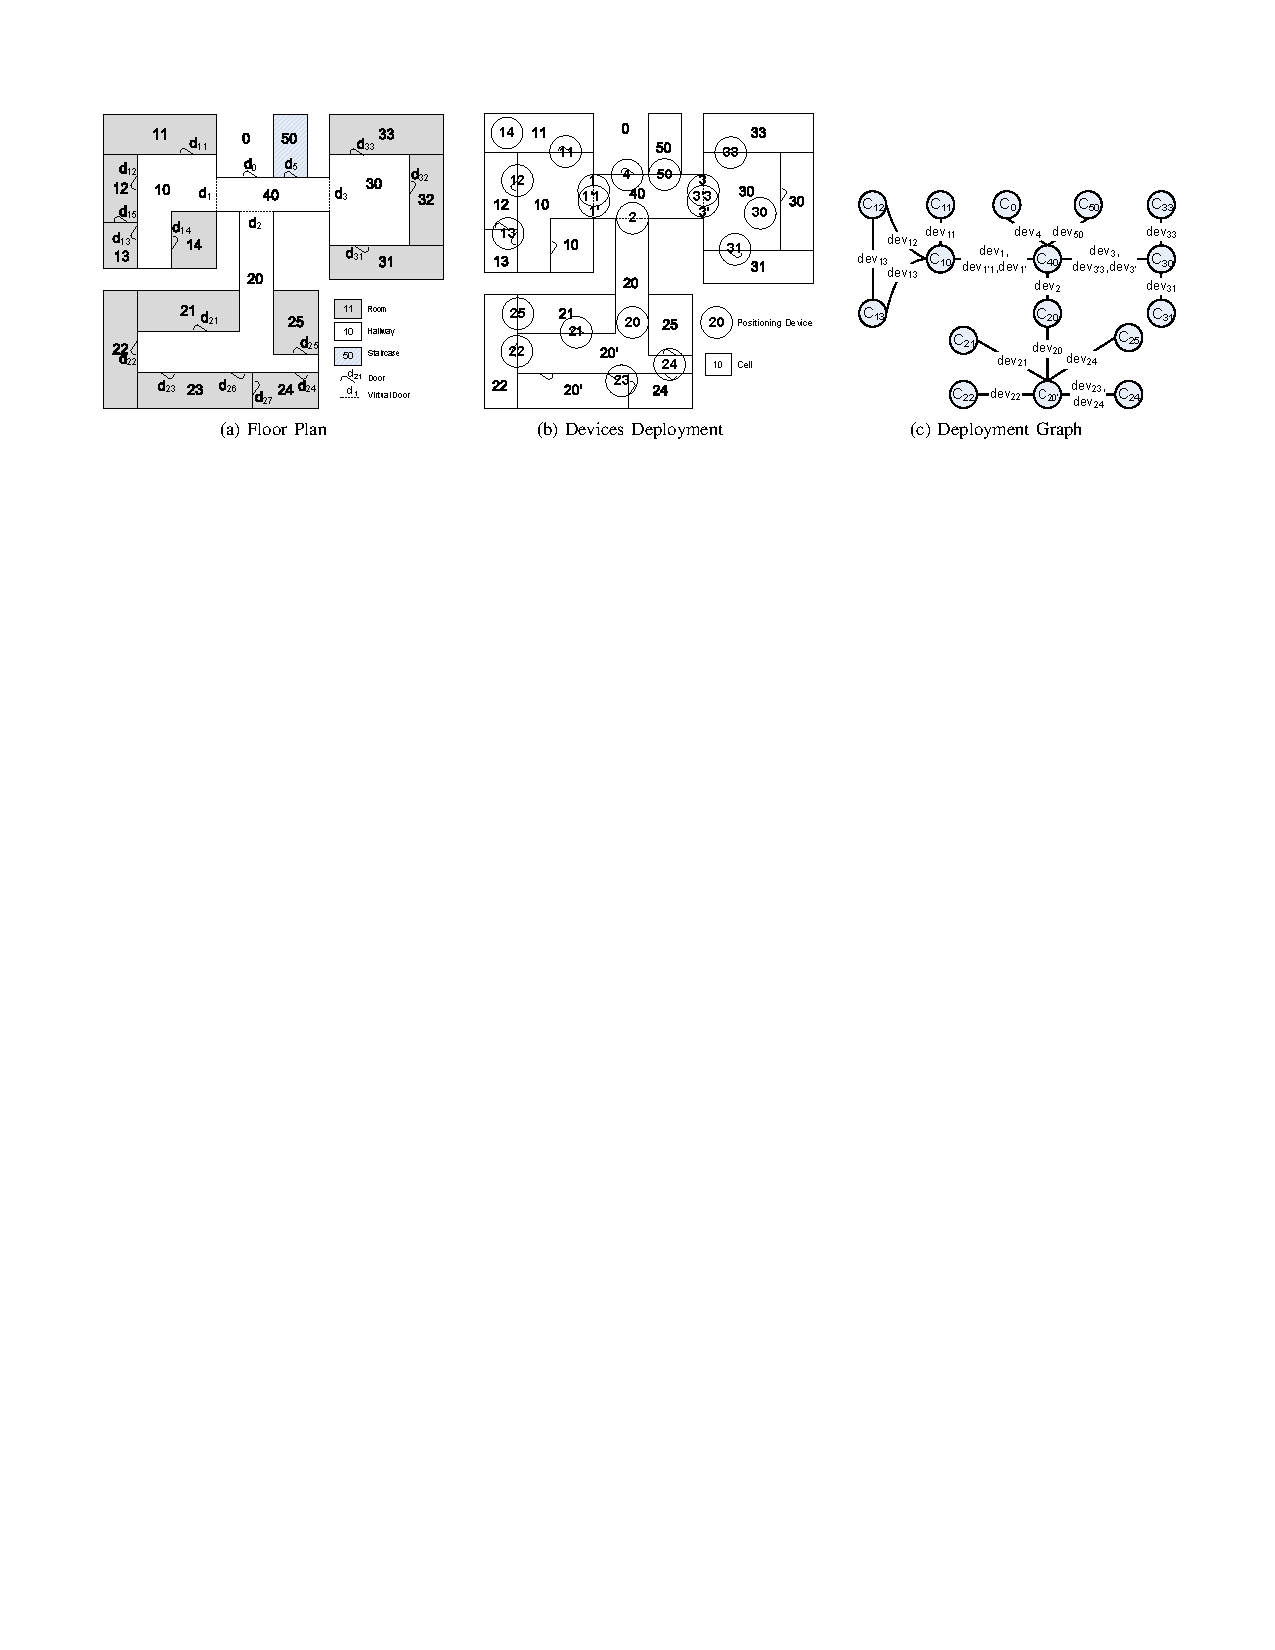
\includegraphics[width=\columnwidth]{figures/2-4/2-4-1.pdf}
\end{figure}

\begin{enumerate}
  \ssize{
  \item $\mn{C2P: C \rightarrow 2^P}$ maps a cell to a set of indoor partitions
  \item $\mn{D2C: D \rightarrow 2^C}$ maps a device to a set of corresponding cells
  \item According to Deployment Graph, for partitioning device, $\mn{D2C(device_{13})} = \{ C_{10},C_{13} \} \cup \{ C_{12},C_{13} \} = \{ C_{10},C_{12},C_{13} \}$
  \item For presence device, $\mn{D2C(device_{25})} = \{ C_{21},C_{22} \}$ as the cells intersect its detection range.
  \item $\mn{D2C: D \rightarrow 2^C}$ is useful as it captures the possible movements of objects.
  }
\end{enumerate}

\end{frame}

%------------------------------------------------

\begin{frame}
\frametitle{Preliminaries: Symbolic Indoor Tracking}

\begin{columns}[c]
  \column{.52\textwidth}
  \begin{figure}[tb]
    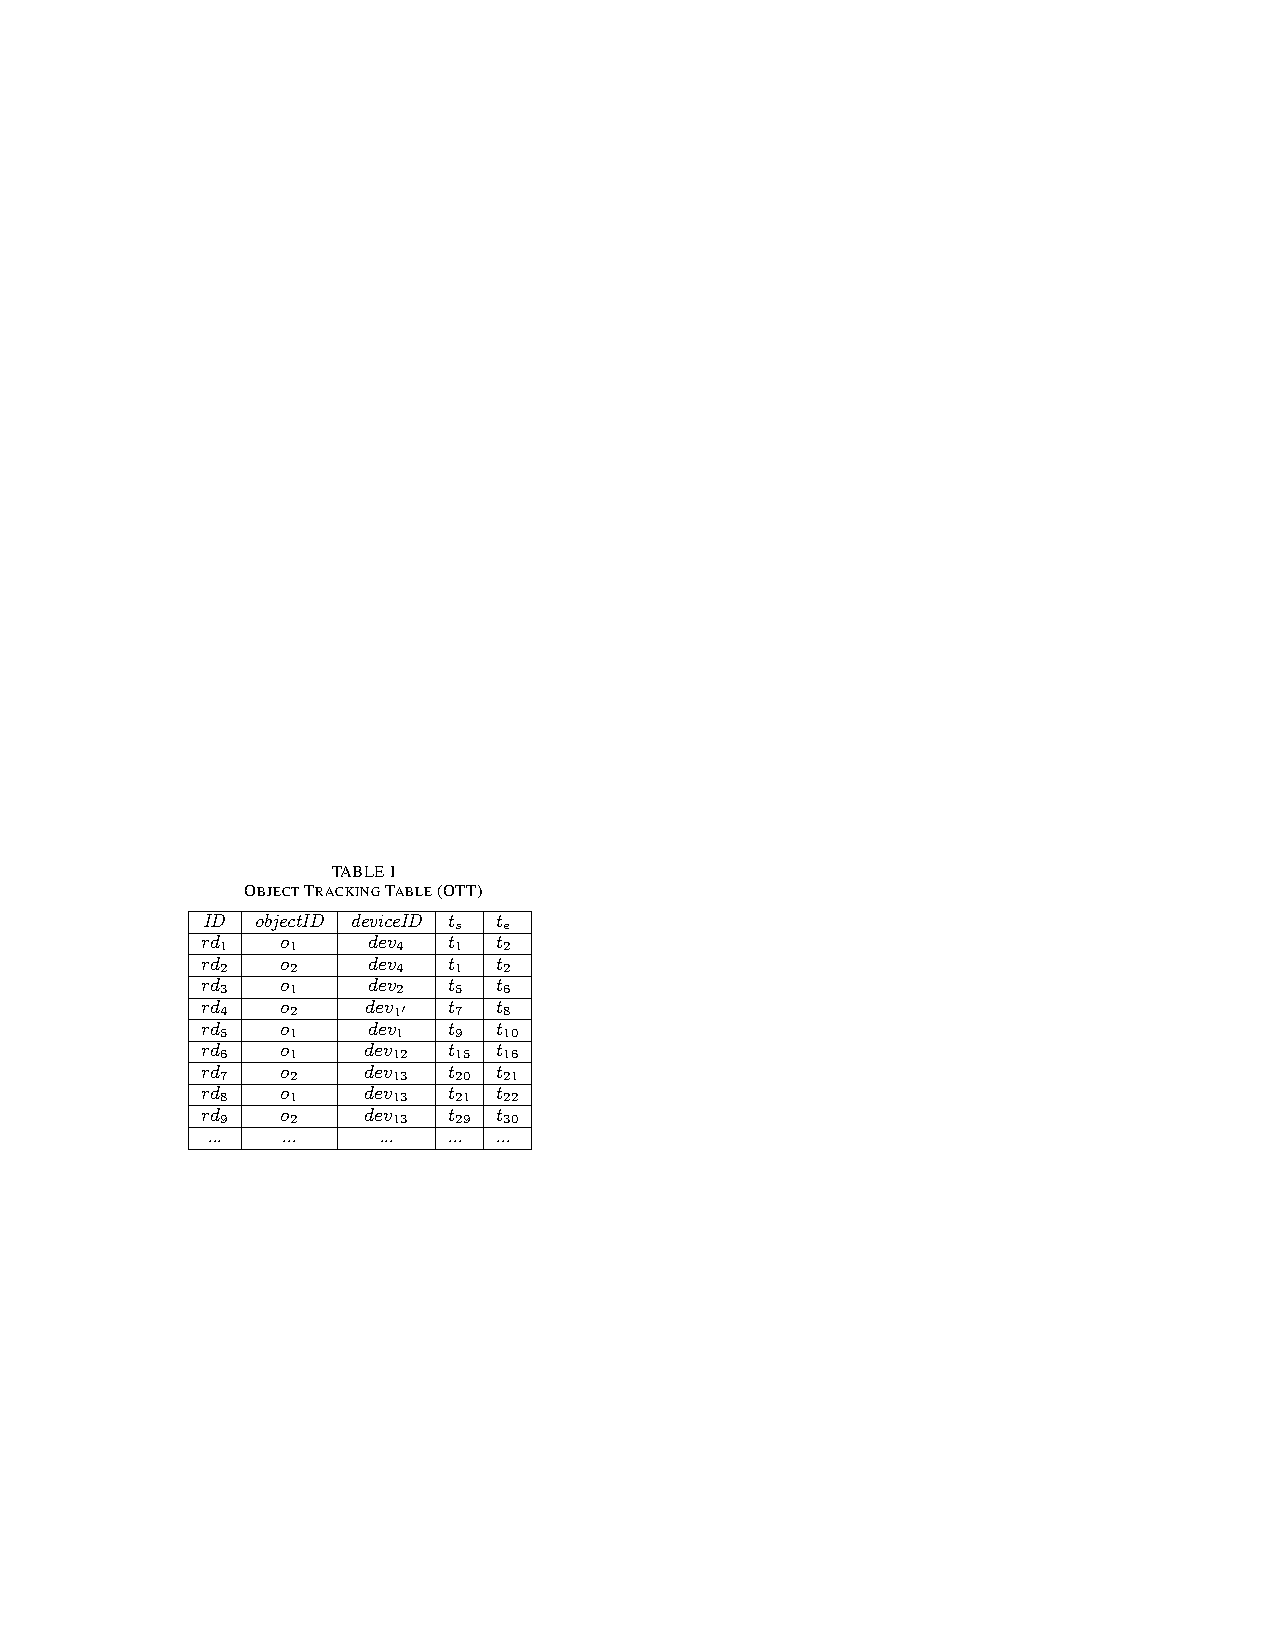
\includegraphics[width=\columnwidth]{figures/2-4/2-4-2.pdf}
  \end{figure}

  \column{.48\textwidth}
  \begin{fitemize}
    \item \conceptbf{Object Tracking Table} $\mn{OTT}$ records the converted trajectories with schema $\mn{(ID, objectID, deviceID, t_s, t_e)}$
    ~\\
    \item a record states that the object $\mn{objectID}$ is observed by the device $\mn{deviceID}$ in the closed interval from time $\mn{t_s}$ to $\mn{t_e}$.
  \end{fitemize}

\end{columns}

\end{frame}

%------------------------------------------------

\begin{frame}
\frametitle{Problem Definitions}

Given an $\mn{OTT}$, it is of interesting to identify object pairs that join w.r.t some specific spatio-temporal join predicate.
\begin{fitemize}
  \item to know all pair of individuals that were probably at the same gate when a particular event (terrorist attack) occurred in a large airport.
\end{fitemize}
~\\
Due to tracking uncertainty, only interested in those objects that satisfy the join predicate with some given probability (specified threshold).
\\~\\
The joins are effectively \emph{self-joins} because all tracking data is contained in a single $\mn{OTT}$.

\end{frame}

%------------------------------------------------

\begin{frame}
\frametitle{Problem Definition I}

\textrm{One can apply a join predicate to a time point to find pairs that join at that particular time point...}
\\~\\
\begin{definition}[\ssize{Probabilistic Threshold Indoor Spatio-temporal Join--PTISSJ}]
  \textrm{
  \ssize{
  Given an $\mn{OTT}$, a join predicate $\mn{P}$, a time point $\mn{t}$, and a threshold value $\mn{M \in (0,1]}$, a probabilistic threshold indoor spatio-temporal join  $\mn{\Join_{P,t,M}(OTT) = \{ (o_i, o_j) | o_i, o_j \in O  \wedge o_i \neq o_j \wedge pr(P(o_i, o_j, t)) >M \}}$, where $\mn{pr(P(o_i,o_j,t))}$ is the \textbf{Timeslice Join Probability} of $\mn{o_i, o_j}$ at time $\mn{t}$, i.e., the probability that predicate $\mn{P(o_i,o_j,t)}$ is true.
  }}
\end{definition}

\end{frame}

%------------------------------------------------

\begin{frame}
\frametitle{Problem Definition II}

\textrm{It's also interesting to know object pairs satisfy the predicate for some consecutive timestamp...}
\\~\\
\begin{definition}[\ssize{Probabilistic Threshold $k$ Indoor Spatio-temporal Join--PT$k$ISSJ}]
  \textrm{
  \ssize{
  Given an $\mn{OTT}$, a join predicate $\mn{P}$, a time interval $\mn{I = [t_m, t_n] (m < n)}$, an integer $\mn{k(0 < k \leq n - m)}$, and a threshold value $\mn{M \in (0,1]}$, a probabilistic $\mn{k}$ threshold indoor spatio-temporal join
  \begin{equation*}
    \begin{split}
    &\mn{\Join_{P,I,k,M}(OTT) = \{ (o_i, o_j) | o_i, o_j \in O \wedge o_i \neq o_j \wedge } \\
    &\mn{\exists s \in m...n -k + 1 (\forall\delta \in 0...k-1 (pr(P(o_i, o_j, t_{s+\delta})) > M)) \} }
    \end{split}
  \end{equation*}
  }}
\end{definition}

\end{frame}

%------------------------------------------------

\begin{frame}
\frametitle{Uncertainty Model for Indoor Tracking}

\textrm{For outdoor moving objects~\cite{cheng2004querying}, \conceptbf{Uncertainty Region}, denoted by $\mn{UR(o_i,t)}$, is a region such that $\mn{o_i}$ must be in this region at time $\mn{t}$.}\\~

In general terms, an object $\mn{o_i}$'s location can be modeled as a random variable $\mn{l}$ associated with a probability density function $\mn{f_{o_i}(l,t)}$ that has non-zero values only in $\mn{o_i}$'s suncertainty region $\mn{UR(o_i, t)}$.~\cite{DBLP:conf/edbt/YangLJ10}

\begin{equation}
  \mn{\int_{l \in UR(o_i,t)} f_{o_i}(l,t) dl = 1}
\end{equation}

\end{frame}

%------------------------------------------------

\begin{frame}
\frametitle{Object State in OTT}

\begin{columns}[c]

\column{.45\textwidth}
\begin{figure}[tb]
  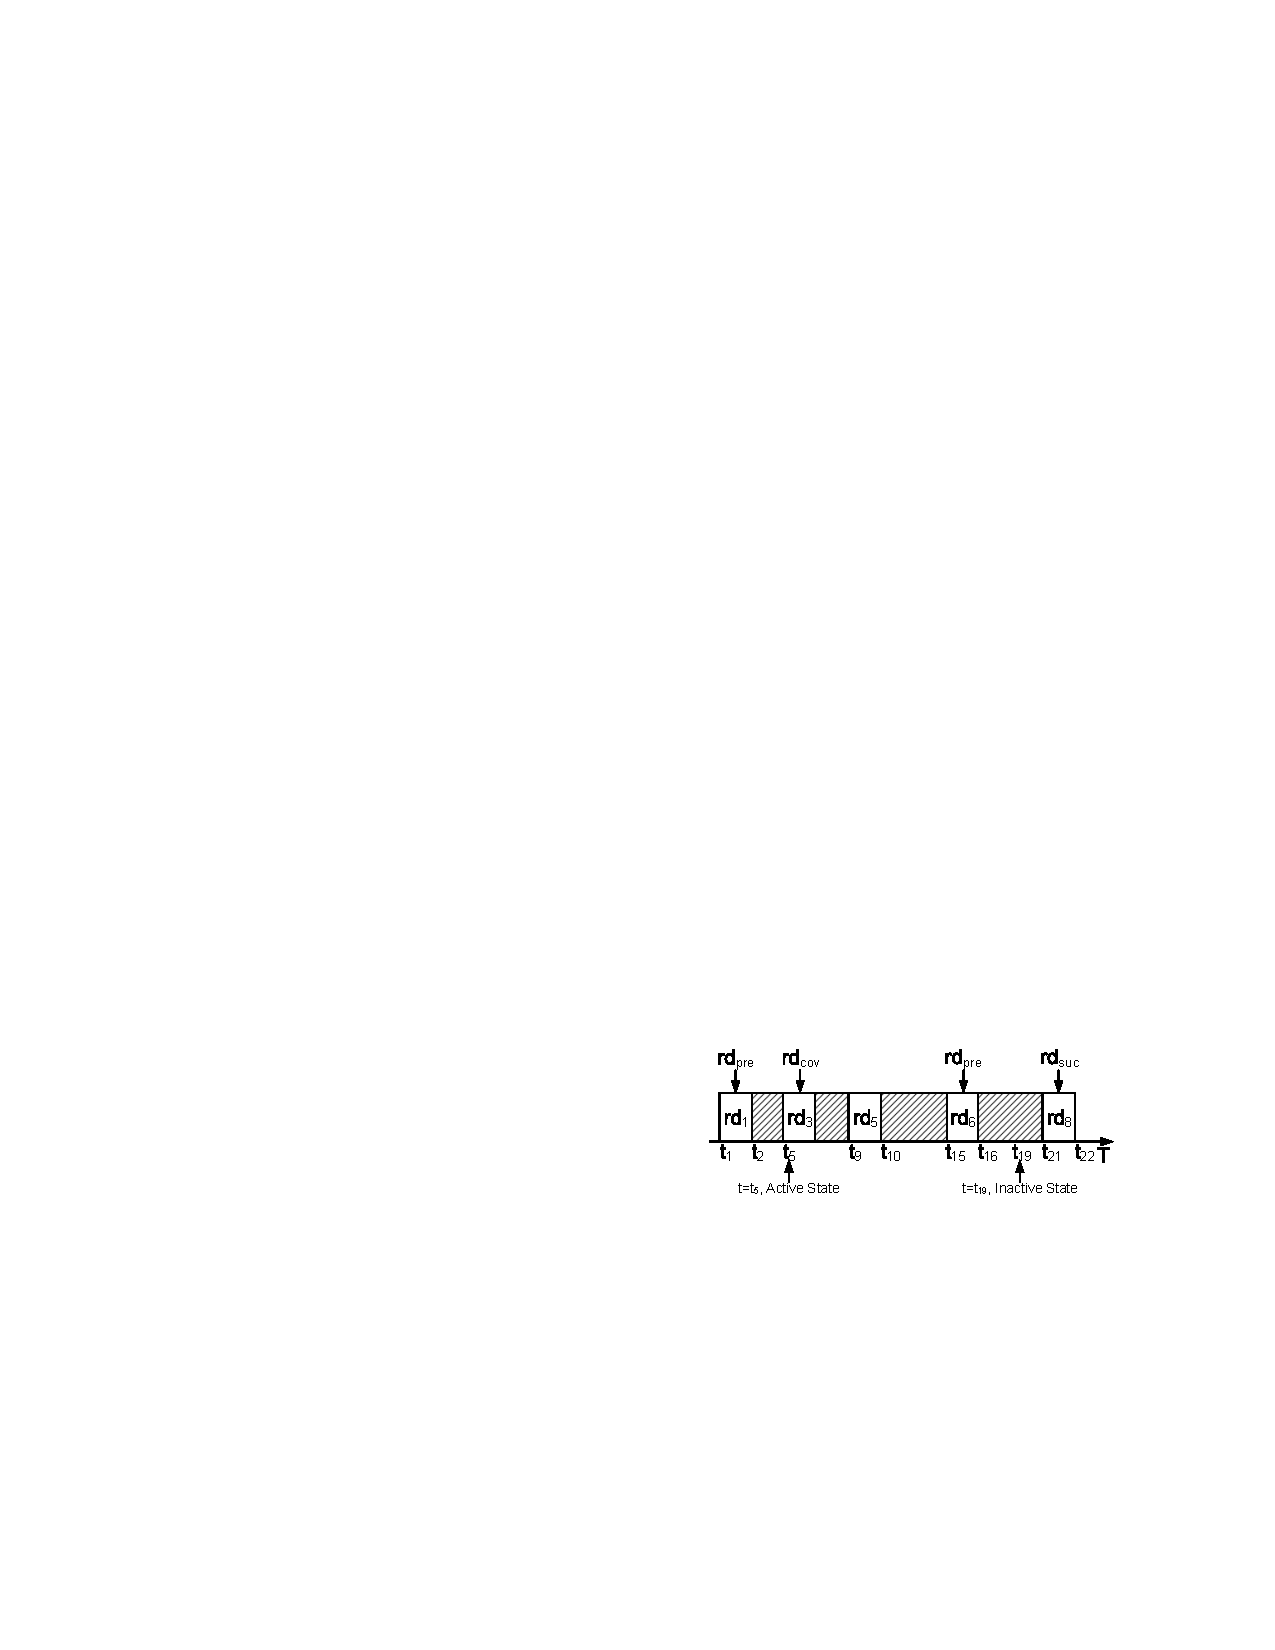
\includegraphics[width=\columnwidth]{figures/2-4/2-4-3.pdf}
\end{figure}

\column{.55\textwidth}
\begin{definition}[Active State]
  \textrm{
  \ssize{
  Given an object $\mn{o_i}$ and a time point $\mn{t}$, if a tracking record $\mn{rd_{cov}}$ is found in $\mn{OTT}$ such that $\mn{rd_{cov}.objectID = o_i}$ and $\mn{t \in [rd_{cov}.t_s, rd_{cov}.t_e]}$, $\mn{o_i}$ is in the \conceptbf{active state} at time $\mn{t}$.
  }}
\end{definition}

\end{columns}

\begin{definition}[Inactive State]
  \textrm{
  \ssize{
  Given an object $\mn{o_i}$ and a time point $\mn{t}$, if no record $\mn{rd_{cov}}$ is found in $\mn{OTT}$, $\mn{o_i}$ is in the \conceptbf{inactive state} at time $\mn{t}$. Instead, two tracking records of $\mn{o_i}$ called $\mn{rd_{pre}}$ and $\mn{rd_{suc}}$, can be found in $\mn{OTT}$, such that they are consecutive in the sense that $\mn{rd_{pre}.t_e < t < rd_{suc}.t_s}$ and there is no record for $\mn{o_i}$ between times $\mn{rd_{pre}.t_e}$ and $\mn{rd_{suc}.t_s}$.
  }}
\end{definition}

\end{frame}

%------------------------------------------------

\begin{frame}
\frametitle{Uncertainty Region in the Active State}

\begin{columns}[c]
  \column{.52\textwidth}
  \vspace{-10pt}
  \begin{figure}[tb]
    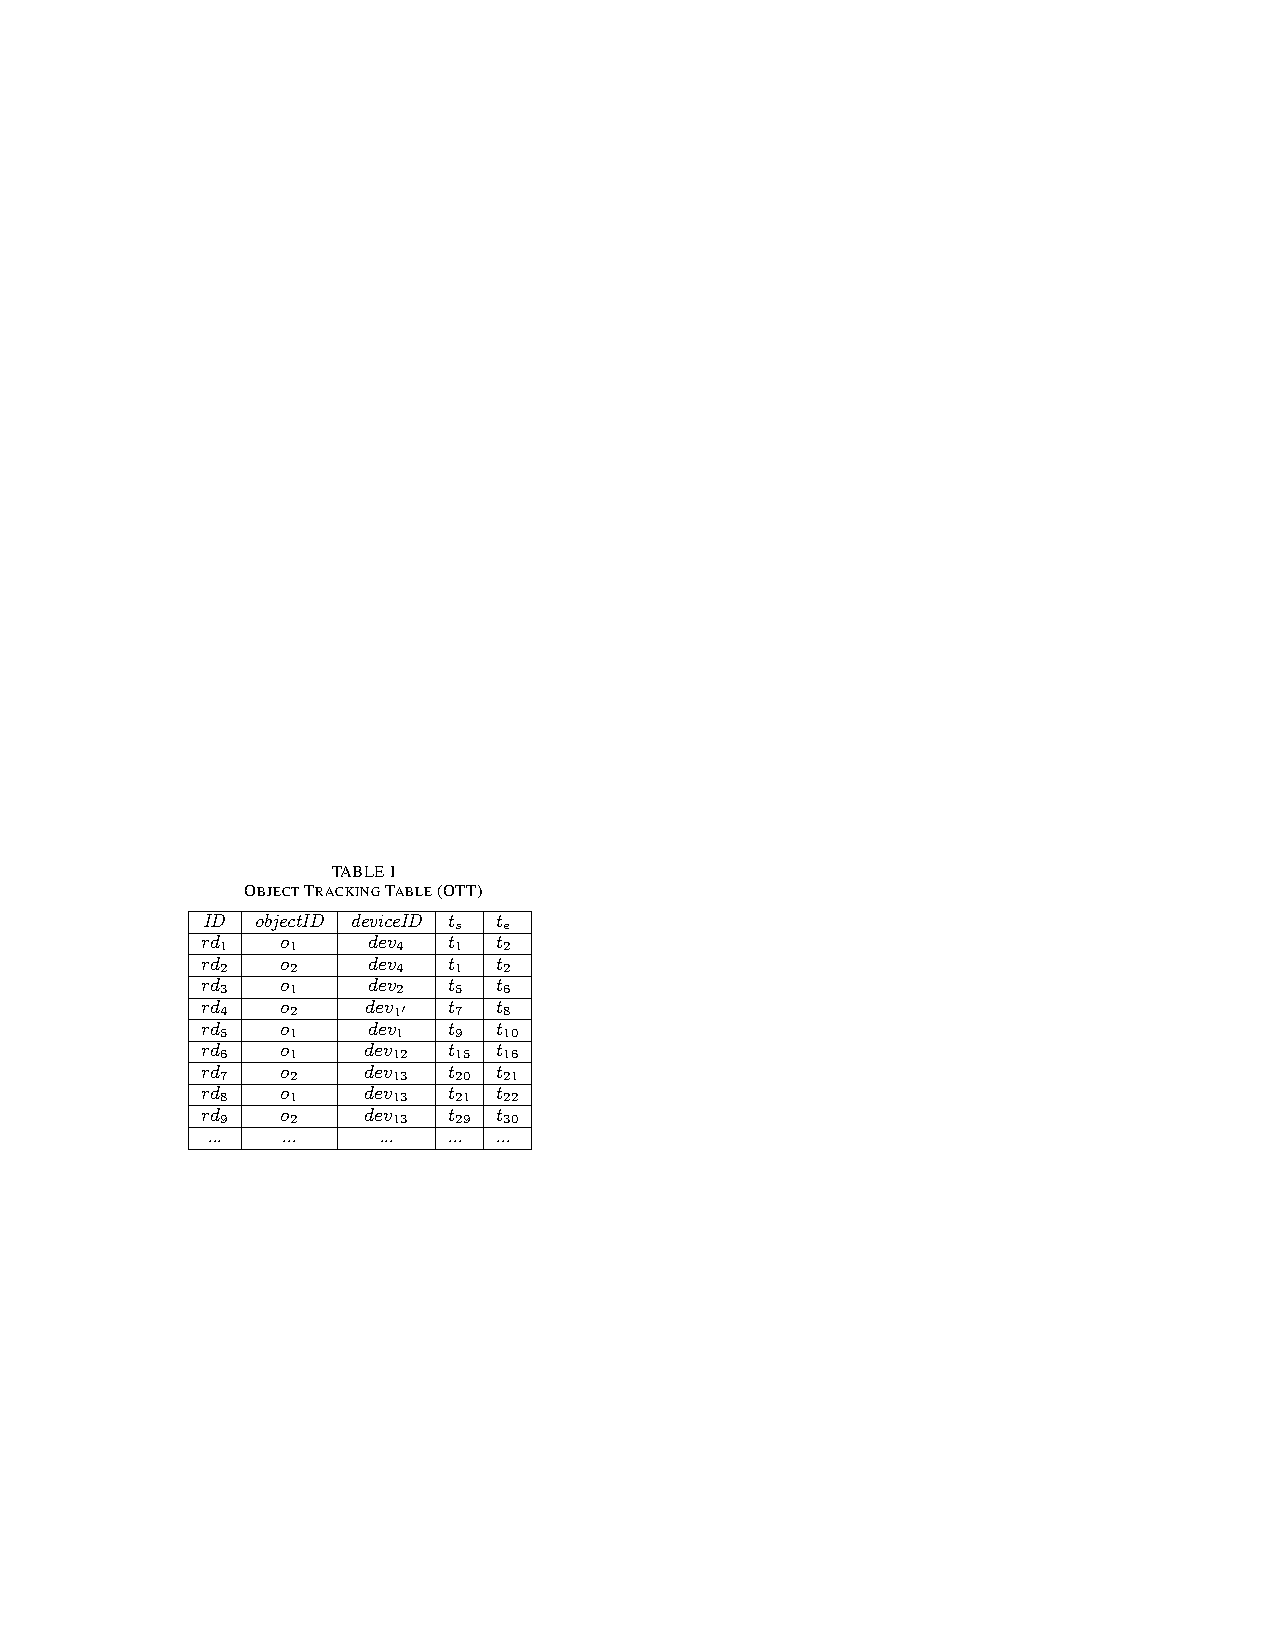
\includegraphics[width=\columnwidth]{figures/2-4/2-4-2.pdf}
  \end{figure}
  \vspace{-15pt}
  \begin{example}
    \textrm{
    \ssize{
    $\mn{t = t_5}$, $\mn{rd_{cov} = rd_3}$ and $\mn{rd_{pre} = rd_1}$, which tells $\mn{o_i}$ left $\mn{dev_4}$'s detection range at time $\mn{t_2}$, and is currently detected by $\mn{dev_2}$.
    }}
  \end{example}

  \column{.48\textwidth}
  \vspace{-10pt}
  \begin{figure}[tb]
    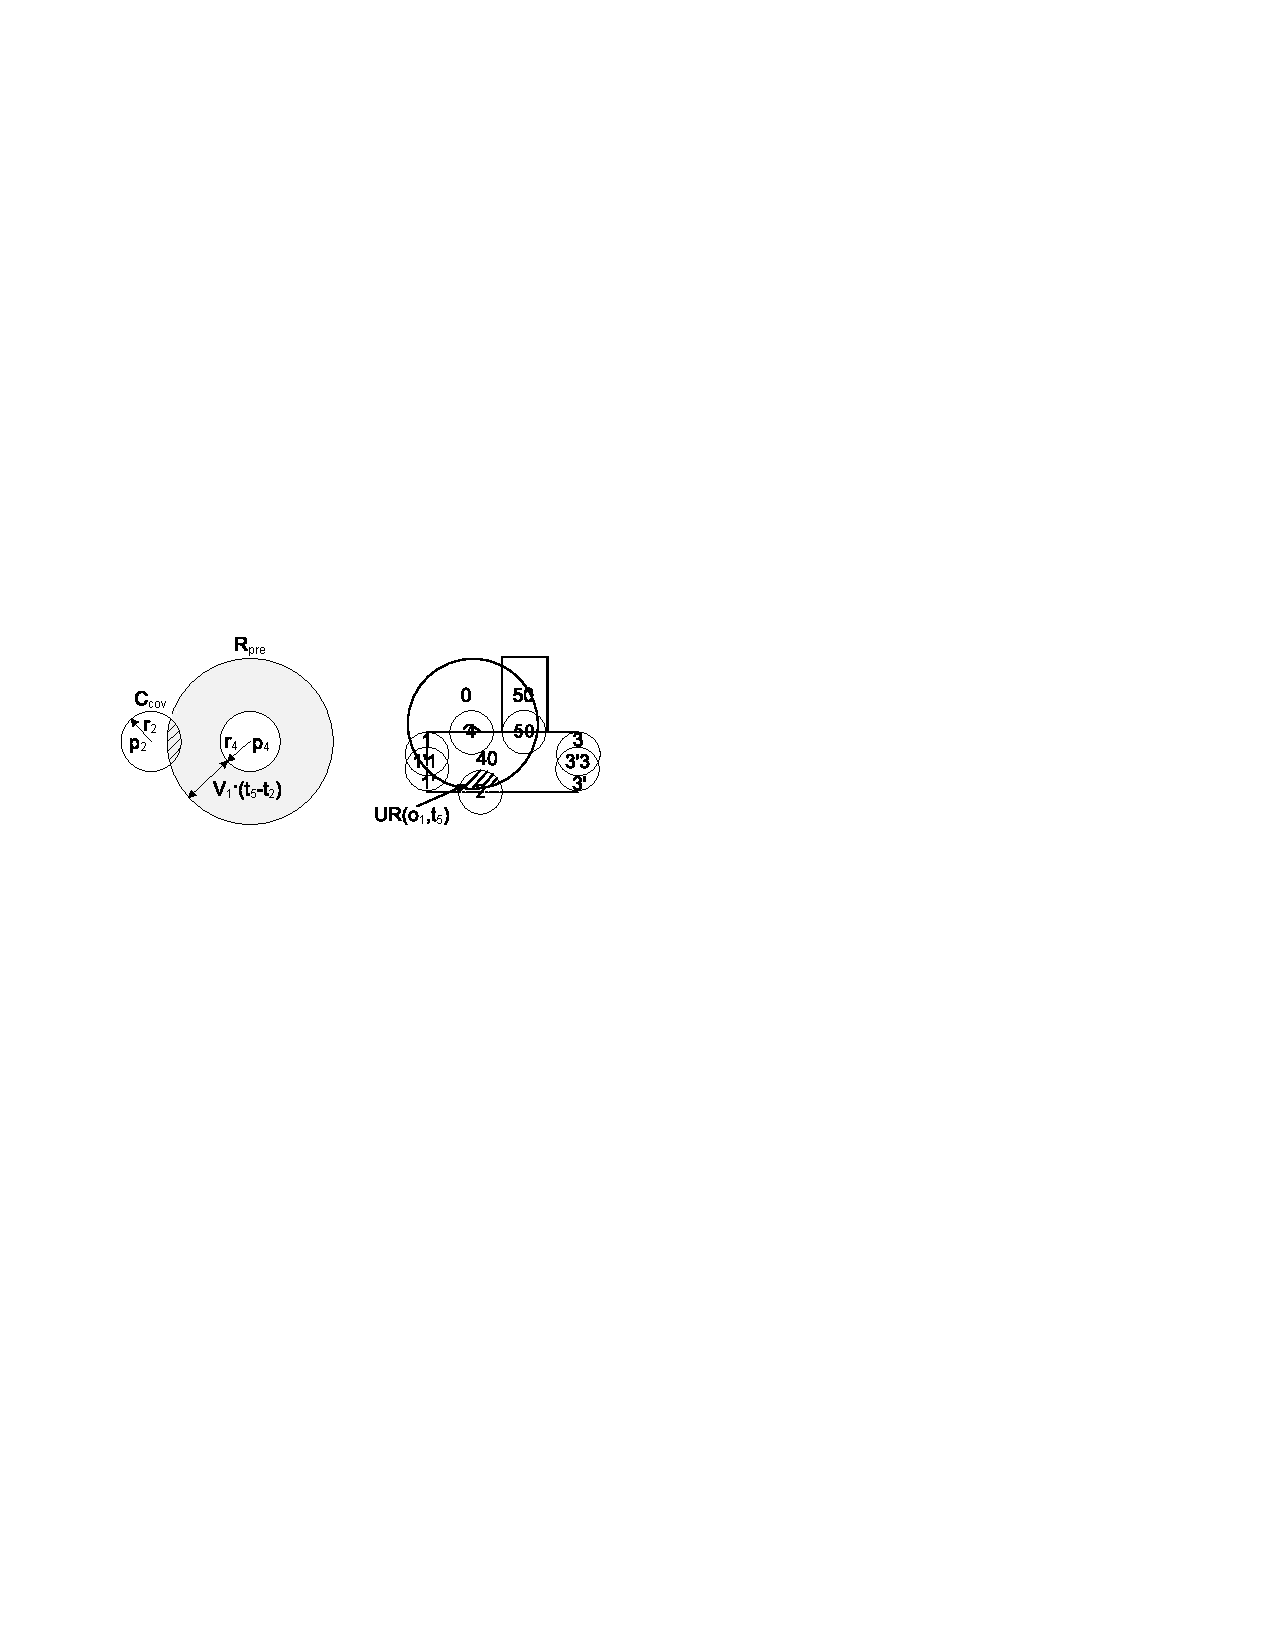
\includegraphics[width=\columnwidth]{figures/2-4/2-4-4.pdf}
  \end{figure}
  \ssize{
  \textbf{Step 1:}
  UR is the detection range of device $\mn{rd_{cov}.deviceID}$, denote as:
  \begin{equation*}
  \begin{split}
    \mn{ C_{cov} = } &\mn { Cir(Loc(rd_{cov}.deviceID), }\\
    &\mn{ Rad(rd_{cov}.deviceID)) }
  \end{split}
  \end{equation*}
  ~\\
  \textbf{Step 2:}
  UR should consider the $\mn{rd_{pre}}$'s \emph{maximum speed bounding ring}(MSBR):
  \tiny{
  \begin{equation*}
  \begin{split}
    &\mn{ UR(o_i, t) = C_{cov} \cap Ring(Loc(rd_{pre}.deviceID), } \\
    &\mn{ Rad(rd_{pre}.deviceID), V_i \cdot (t - rd_{pre}.t_e) ) }
  \end{split}
  \end{equation*}
  }
  }
\end{columns}

\end{frame}

%------------------------------------------------

\begin{frame}
\frametitle{Uncertainty Region in the Inactive State}

\begin{columns}[c]

  \column{.52\textwidth}
  \vspace{-10pt}
  \begin{figure}[tb]
    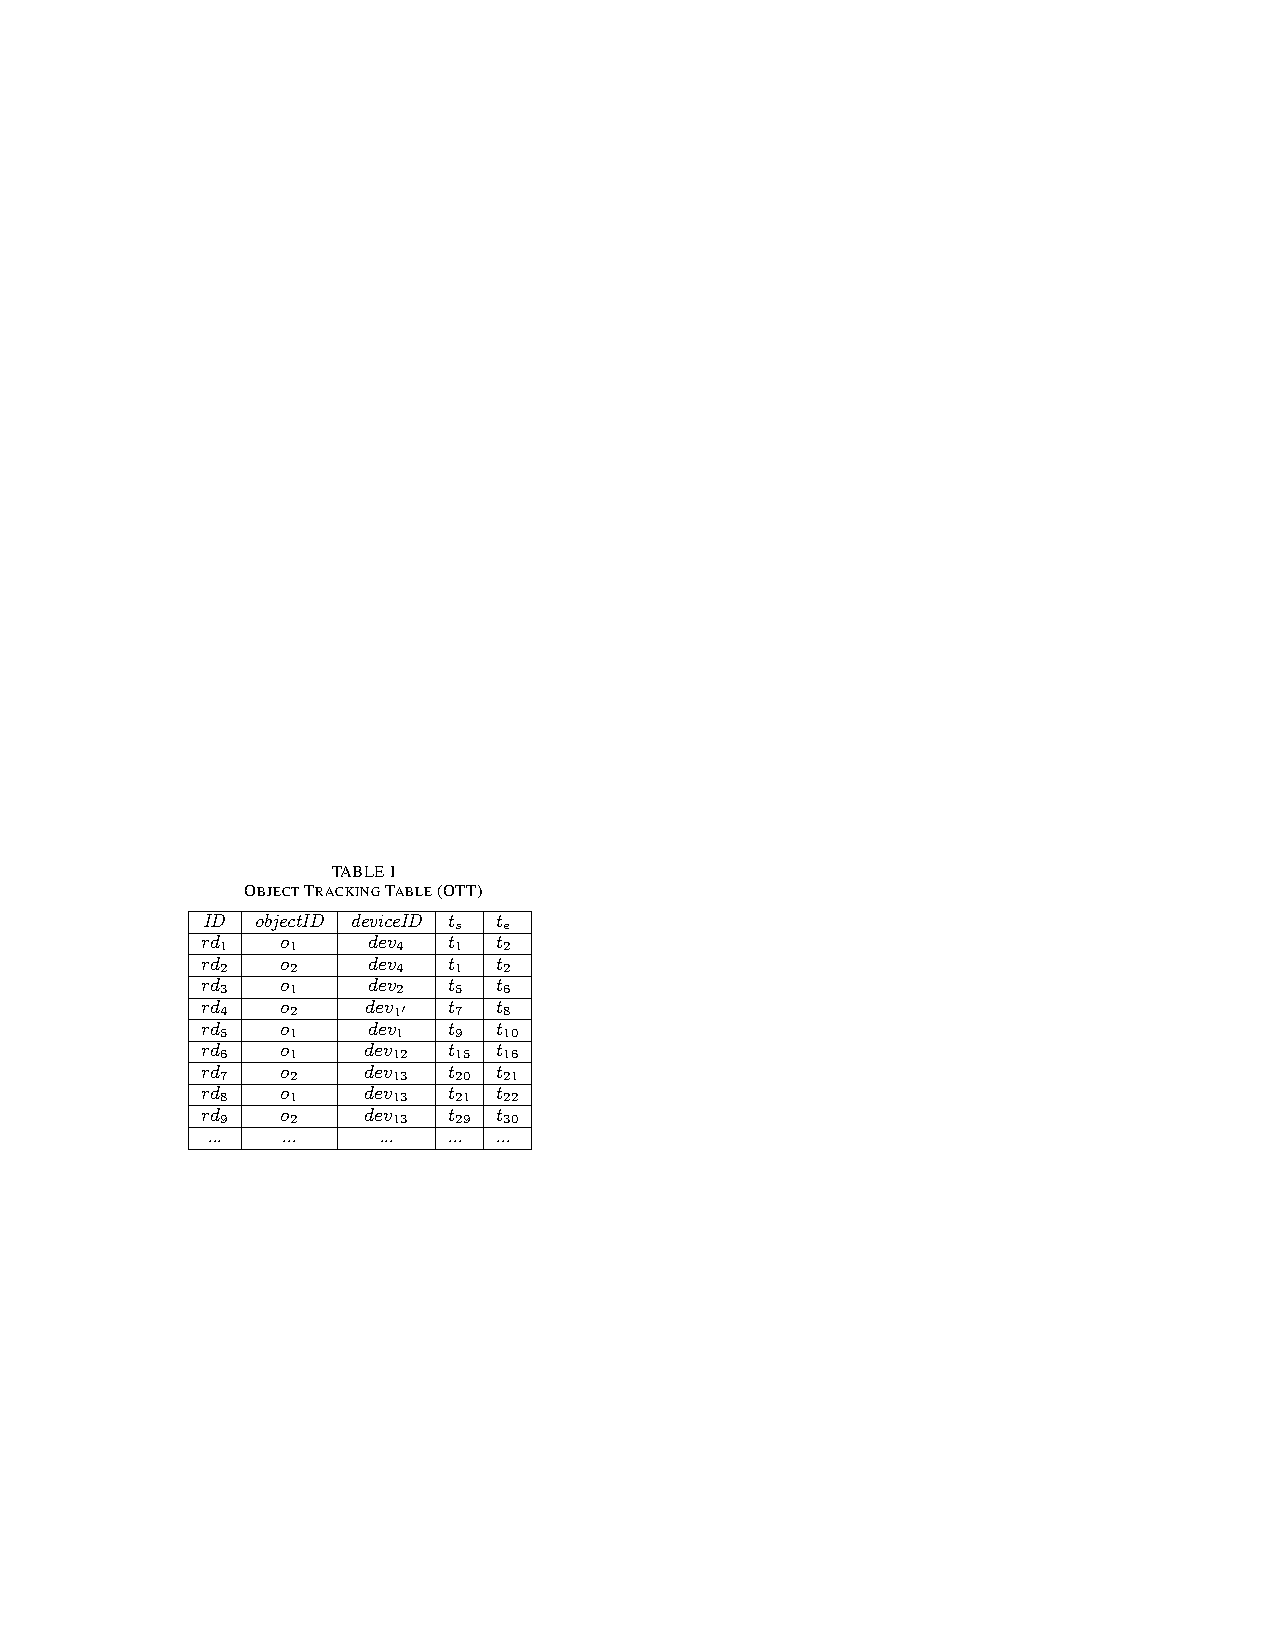
\includegraphics[width=\columnwidth]{figures/2-4/2-4-2.pdf}
  \end{figure}
  \vspace{-15pt}
  \begin{example}
    \textrm{
    \ssize{
    $\mn{t = t_{19}}$, $\mn{rd_{pre} = rd_6}$ and $\mn{rd_{suc} = rd_8}$, since $\mn{rd_6.t_e = t_{16} < t_{19} < rd_8.t_s = t_{21}}$. we have $\mn{dev_p = dev_{12}}$ and $\mn{dev_s = dev_{13}}$
    }}
  \end{example}

  \column{.48\textwidth}
  \vspace{-10pt}
  \begin{figure}[tb]
    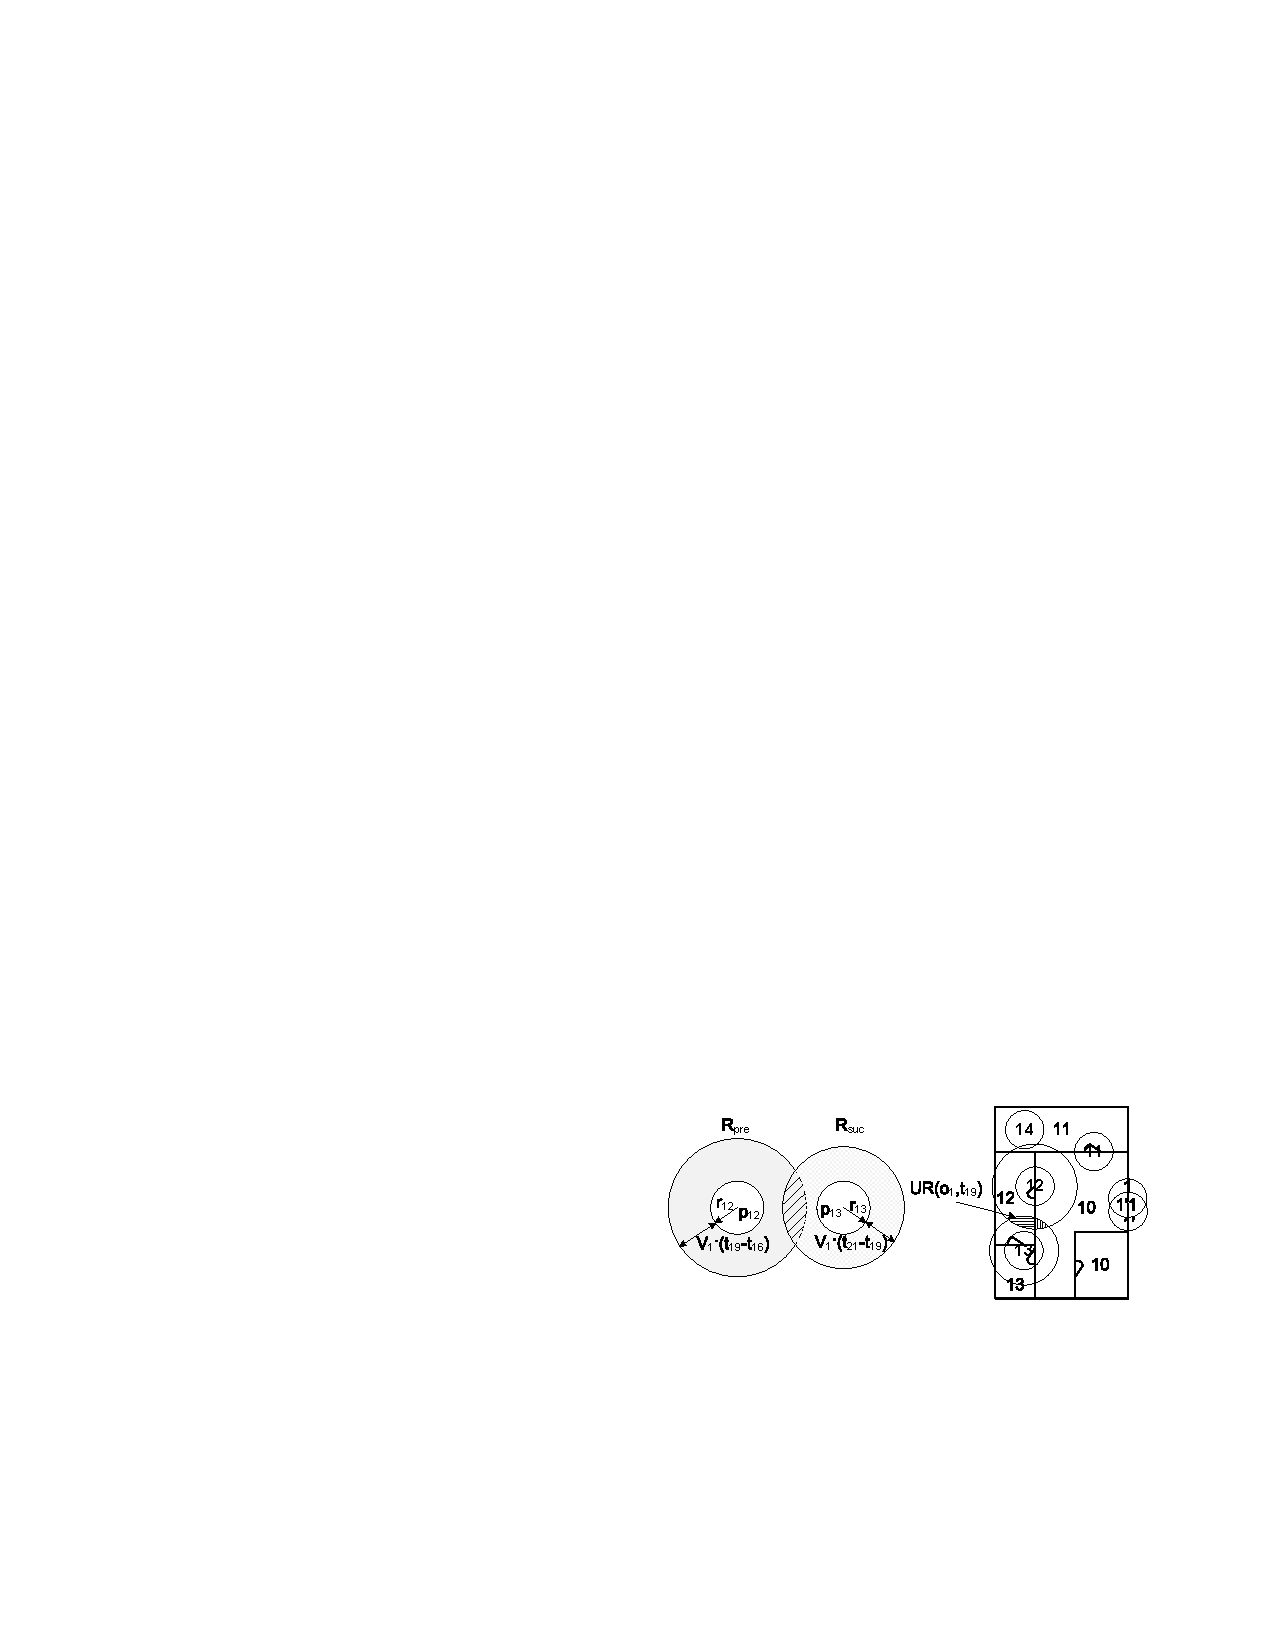
\includegraphics[width=\columnwidth]{figures/2-4/2-4-5.pdf}
  \end{figure}
  \ssize{
  \textbf{Step 1:}
  Determine the possible cells in which the object can be in the inactive period:
  \begin{equation*}
    \mn{ Cells_{mid} = D2C(dev_p) \cup D2C(dev_s)}
  \end{equation*}
  ~\\
  \textbf{Step 2:}
  UR is constrained by two \emph{maximum speed bounding ring}(MSBR)s of $\mn{rd_{pre}}$ and $\mn{rd_{suc}}$:
  \tiny{
  \begin{equation*}
  \begin{split}
    \mn{ UR(o_i, t) = \bigcup_{c \in Cells_{mid}} c \cap R_{pre} \cap R_{suc} }
  \end{split}
  \end{equation*}
  }
  }
\end{columns}

\end{frame}
